\chapter{Linear regression and regularization}
\label{ch:linear-regression}

\begin{learningobjectives}
After this chapter, you should be able to:
\begin{itemize}
  \item derive least squares from an affine prediction rule and squared loss;
  \item explain projection, identifiability, conditioning, and stable numerical
  solution;
  \item distinguish prediction, coefficient interpretation, and statistical
  uncertainty;
  \item distinguish ridge, lasso, and elastic-net regularization; and
  \item evaluate a regression pipeline using residual and out-of-sample
  evidence while measuring numerical and computational performance.
\end{itemize}
\end{learningobjectives}

\begin{chapterconnection}
Chapter~\ref{ch:supervised-contract} fixed the population, feature cutoff,
target, split, and baseline. We can now study model classes without silently
changing the question. The affine map introduced here will recur in logistic
regression, support-vector machines, and neural networks.
\end{chapterconnection}

\section{From astronomical observations to a general model}

Least squares arose from a scientific problem that still feels modern: more
noisy measurements were available than unknown parameters, and no parameter
choice satisfied every equation exactly. Adrien-Marie Legendre published the
method in 1805 as part of work on comet orbits. Carl Friedrich Gauss published
a probabilistic treatment in 1809 and stated that he had used the principle
earlier.\footnote{A.-M. Legendre, \emph{Nouvelles m\'ethodes pour la
d\'etermination des orbites des com\`etes}, 1805; C. F. Gauss, \emph{Theoria
motus corporum coelestium}, 1809. Legendre's appendix is the first published
account; Gauss reported use dating to 1795.}

The word regression entered statistics later through nineteenth-century studies
of heredity. Its historical biological interpretation should not be confused
with the modern mathematical definition. Today linear regression is a family
of projection, estimation, prediction, and uncertainty procedures. These uses
share algebra but require different assumptions.

The model remains important not because all relationships are straight lines,
but because it is transparent enough to expose the entire chain: representation,
loss, geometry, probability, numerical linear algebra, evaluation, and
deployment. It is also the local building block of many nonlinear methods.

\section{The affine predictor}

For $x\in\mathbb{R}^p$, an affine predictor has the form
\[
f_{w,b}(x)=w^Tx+b.
\]
The intercept permits a nonzero prediction at the coordinate origin. Calling
this model ``linear'' is conventional; mathematically it is affine unless the
intercept is absorbed into an augmented feature vector.

With design matrix $X\in\mathbb{R}^{n\times p}$ and target vector
$y\in\mathbb{R}^n$, ordinary least squares minimizes
\[
J(w,b)=\frac{1}{n}\sum_{i=1}^n(y_i-w^Tx_i-b)^2.
\]
Squared loss penalizes large residuals strongly and targets the conditional mean
under the population risk. That property is useful only when the mean and the
cost implied by squared error match the task.

\section{One feature exposes the algebra}

For observations $(x_i,y_i)$ and $\widehat y_i=b+wx_i$, minimize
\[
Q(b,w)=\sum_{i=1}^n[y_i-(b+wx_i)]^2.
\]
The first-order equations are
\[
\sum_i(y_i-b-wx_i)=0,
\qquad
\sum_i x_i(y_i-b-wx_i)=0.
\]
The first implies that the fitted line passes through $(\bar x,\bar y)$. After
centering, the solution is
\[
\widehat w=
\frac{\sum_i(x_i-\bar x)(y_i-\bar y)}
     {\sum_i(x_i-\bar x)^2},
\qquad
\widehat b=\bar y-\widehat w\bar x.
\]
Thus the slope is sample covariance divided by sample variance when the same
normalizing convention is used. If every $x_i$ is equal, the denominator is
zero: the sample contains no information about change in $y$ with $x$.

Residuals satisfy
\[
\sum_i e_i=0,
\qquad
\sum_i x_ie_i=0
\]
when an intercept and slope are fitted. These are orthogonality statements, not
evidence that residuals are independent, Gaussian, or scientifically harmless.

\conceptcheck{If mass is converted from grams to kilograms, how do slope and
intercept coordinates change? Why are fitted values unchanged when the
conversion is performed consistently?}

\section{Projection and identifiability}

After including an intercept column, write the design matrix as $A$. The fitted
vector $A\widehat\theta$ is the orthogonal projection of $y$ onto the column
space of $A$. At an optimum the residual $r=y-A\widehat\theta$ satisfies
$A^Tr=0$. This geometric statement remains meaningful when coefficients are
not unique.

\begin{theorem}[Least squares is orthogonal projection]
\label{thm:least-squares-projection}
Let $\mathcal C(A)$ be the column space of a real matrix $A$. A vector
$\widehat y=A\widehat\theta$ minimizes $\lVert y-Av\rVert_2^2$ over all $v$
if and only if its residual $r=y-\widehat y$ is orthogonal to
$\mathcal C(A)$, equivalently $A^Tr=0$. The fitted vector $\widehat y$ is
unique even when the coefficient vector $\widehat\theta$ is not.
\end{theorem}

\begin{proof}
Suppose first that $r\perp\mathcal C(A)$. For any candidate $Av$, the vectors
$r=y-A\widehat\theta$ and $A\widehat\theta-Av$ are orthogonal. Pythagoras gives
\[
\lVert y-Av\rVert_2^2
=\lVert y-A\widehat\theta\rVert_2^2
+\lVert A\widehat\theta-Av\rVert_2^2.
\]
The right side is minimized at the projected vector. Conversely, if a
minimizer had $A^Tr\ne0$, then for $d=A^Tr$ the directional derivative of
$\lVert y-A(\widehat\theta+td)\rVert_2^2$ at $t=0$ would be
$-2\lVert A^Tr\rVert_2^2<0$, contradicting minimality. Orthogonal projection
onto a finite-dimensional subspace is unique, although a rank-deficient $A$
can map several coefficient vectors to that same projection.
\end{proof}

The Pythagorean identity separates unexplained residual length from the extra
error caused by choosing another vector in the same model space. It is also a
unit test: a computed least-squares residual should satisfy $A^Tr\approx0$ up
to a tolerance justified by scale and conditioning.

If $A$ has full column rank, the normal equations give
\[
\widehat\theta=(A^TA)^{-1}A^Ty.
\]
Software should not explicitly form the inverse. QR or singular-value methods
are generally more stable, while iterative methods are useful at larger scale.
When columns are linearly dependent, multiple coefficient vectors produce the
same fitted values. Prediction may remain defined while individual coefficient
interpretations do not.

The Moore-Penrose pseudoinverse $A^+$ gives the minimum-Euclidean-norm solution
$\widehat\theta=A^+y$ when the system is rank deficient. That convention makes
a coefficient vector unique, but it does not make the individual coefficients
scientifically identified. The choice comes from an algebraic preference among
equally fitting solutions.

Figure~\ref{fig:regression-geometry} shows the same fit in three coordinate
systems. Data space displays predictions and residual segments. Residual space
reveals structure hidden by one summary. Parameter space shows that least
squares is an optimization problem with a geometric minimum. No single panel
is a substitute for the other two.

\begin{figure}[htbp]
  \centering
  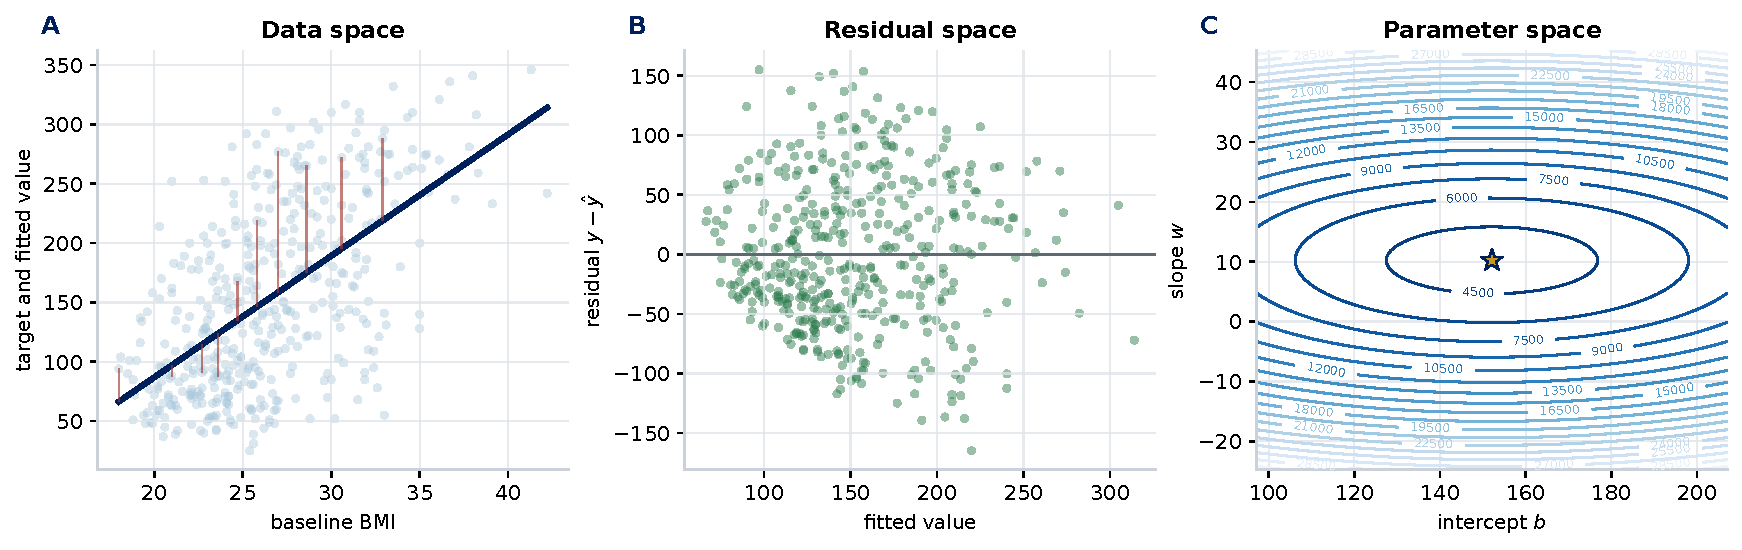
\includegraphics[width=\textwidth]{figures/generated/regression-geometry.pdf}
  \caption{One-feature ordinary least squares on the course diabetes table.
  The coefficients are computed with \code{numpy.linalg.lstsq}; the same
  predictions generate the data-space line, residual plot, and MSE contours.}
  \label{fig:regression-geometry}
\end{figure}

\conceptcheck{Two columns record temperature in Celsius and Fahrenheit. What
happens to rank, fitted values, and the uniqueness of their separate
coefficients when an intercept is present?}

\section{Stable solution is a numerical question}

The symbolic expression
\[
\widehat\theta=(A^TA)^{-1}A^Ty
\]
is useful for derivation but is usually a poor algorithm. Forming $A^TA$ squares
the condition number, and explicitly computing an inverse adds work and error.
QR factorization solves the full-rank least-squares problem without that
inverse. Singular-value decomposition exposes rank and supplies a stable
pseudoinverse. Iterative methods become important when $A$ is too large or
sparse for a direct factorization.

Conditioning asks how much the solution can change under small perturbations to
data or arithmetic. If two columns are nearly dependent, fitted predictions may
be stable in the observed region while their separate coefficients change
dramatically. More floating-point precision does not fix weak statistical
identification.

Standardization can improve numerical conditioning, but it is a fitted
transformation. Means and scales belong to the training fold and serialized
pipeline. Chapter~\ref{ch:gradient-descent} studies how this same conditioning
controls iterative convergence.

\begin{professionalbox}
Use a least-squares routine that reports or permits inspection of rank and
singular values. Record the feature schema and units. Treat a large condition
number as evidence requiring investigation, not as a warning to suppress.
\end{professionalbox}

\subsection{Computational cost belongs to the algorithm, not just the model}

For dense $A\in\mathbb{R}^{n\times p}$ with $n\ge p$, a QR-based solve costs
on the order of $np^2$ arithmetic operations and stores the design or a
factorization of comparable scale. Forming $A^TA$ costs on the same leading
order but worsens conditioning; explicitly inverting it is neither necessary
nor the preferred benchmark. When $p$ is modest and repeated targets share the
same design, a factorization can be reused. When $A$ is large and sparse,
matrix-vector products and iterative solvers may be the only viable interface.

Measure wall time after a warmup and across repeated fits, but also record
problem shape, sparsity, numerical precision, thread count, and peak memory.
Prediction cost for a dense linear model is $O(mp)$ for $m$ new rows and is
often dominated by preprocessing or data movement. Time the complete pipeline
and the estimator separately before deciding what to optimize.

\section{Prediction assumptions differ from inferential assumptions}

A common stochastic model is
\[
Y=X\beta+\varepsilon,
\qquad \mathbb{E}[\varepsilon\mid X]=0.
\]
Under homoscedastic uncorrelated errors with variance $\sigma^2$, ordinary least
squares is the best linear unbiased estimator in the Gauss-Markov sense. This
is a comparison within linear unbiased estimators, not a claim that OLS is best
among every possible predictor.

If errors are conditionally Gaussian, least squares is also maximum likelihood.
Gaussian errors are not required to compute coefficients or predictions. They
support particular likelihood and finite-sample inference results. Independence,
linearity of the conditional mean, constant variance, measurement quality, and
sampling design remain separate assumptions.

For full-rank fixed design,
\[
\operatorname{Var}(\widehat\beta\mid X)=\sigma^2(X^TX)^{-1}.
\]
Uncertainty grows in weakly supported directions. A confidence interval for a
mean response, a prediction interval for a new outcome, and variability of the
entire fitted procedure under new training samples are different objects. A new
outcome interval includes irreducible outcome variation and is therefore wider
than an interval for the conditional mean under the same model.

\begin{theorem}[Gauss-Markov]
\label{thm:gauss-markov}
In the fixed-design model $y=A\beta+\varepsilon$, assume $A$ has full column
rank, $\mathbb{E}[\varepsilon\mid A]=0$, and
$\operatorname{Var}(\varepsilon\mid A)=\sigma^2I$. Among estimators linear in
$y$ and unbiased for every $\beta$, ordinary least squares has minimum
covariance: for any such $\widetilde\beta$,
$\operatorname{Var}(\widetilde\beta\mid A)-
\operatorname{Var}(\widehat\beta_{\mathrm{OLS}}\mid A)$ is positive
semidefinite.
\end{theorem}

\begin{proof}
Write $C_0=(A^TA)^{-1}A^T$, so
$\widehat\beta_{\mathrm{OLS}}=C_0y$. Any linear estimator $Cy$ is unbiased for
every $\beta$ exactly when $CA=I$. Set $D=C-C_0$. Then $DA=0$, and therefore
$C_0D^T=(A^TA)^{-1}A^TD^T=0$. Consequently
\[
\operatorname{Var}(Cy\mid A)
=\sigma^2(C_0+D)(C_0+D)^T
=\sigma^2C_0C_0^T+\sigma^2DD^T.
\]
The final term is positive semidefinite. This proves the comparison. Notice
what the proof does not say: it does not compare nonlinear or biased
estimators, and it does not establish that the model assumptions hold.
\end{proof}

\begin{misconceptionbox}
\textbf{Misconception:} a small coefficient $p$-value proves that changing the
feature will change the outcome. \textbf{Correction:} the inferential statement
is conditional on a statistical model and sampling design. An intervention
claim additionally needs causal identification; practical predictive value
needs out-of-sample evidence.
\end{misconceptionbox}

\section{Basis expansion changes the feature map}

Polynomial regression remains linear in its fitted coefficients. A map
$\phi(x)=(1,x,x^2,\ldots,x^d)$ creates a richer function
$f(x)=w^T\phi(x)$. Interactions can represent joint effects. The flexibility
comes from the basis, not from abandoning linear estimation.

High-degree bases can be poorly conditioned and unstable outside the observed
range. Every basis term must be generated identically during training and
inference. Feature names, order, units, and transformation parameters therefore
belong to the artifact contract.

\section{Regularization chooses among fitting rules}

Ridge regression minimizes
\[
\widehat R(w)+\lambda\lVert w\rVert_2^2,
\]
shrinking correlated or weakly identified coefficients and usually improving
conditioning. Lasso uses $\lambda\lVert w\rVert_1$ and can set coefficients
exactly to zero. Elastic net combines both penalties.

Regularization trades empirical fit for a restriction on the solution. The
penalty depends on feature scale, so scaling and whether the intercept is
penalized are part of the definition. A lasso-selected variable set is not an
automatic list of scientific causes; selection can be unstable among correlated
features.

For a centered design, the ridge solution is
\[
\widehat w_{\mathrm{ridge}}
=(X^TX+\lambda I)^{-1}X^Ty.
\]
In the singular-vector directions of $X$, ridge shrinks most strongly where the
data contain least information. It replaces division by a small squared
singular value $s_j^2$ with division by $s_j^2+\lambda$. This connects
statistical stabilization to numerical conditioning. Under a Gaussian prior on
coefficients and Gaussian observation model, the same expression is a maximum
a posteriori estimate, but that interpretation requires its probability model.

\begin{misconceptionbox}
\textbf{Misconception:} regularization is needed only when a model visibly
overfits. \textbf{Correction:} it can also stabilize an ill-conditioned
problem, encode a preference among many solutions, and improve performance
under finite samples. Its strength must still be chosen inside evaluation.
\end{misconceptionbox}

\section{Residuals are structured evidence}

A residual $e_i=y_i-\widehat y_i$ retains sign, scale, and context. Plot it
against predictions, major features, time, and groups. Curvature can reveal
missing structure; a fan shape can reveal changing conditional variance;
clusters can reveal omitted batches; isolated points can dominate squared loss.

Aggregate error should include units and a distribution, not only a mean.
Compare mean absolute error, root mean squared error, and relevant quantiles.
Inspect error by scientifically meaningful subgroup. Prediction intervals,
confidence intervals for parameters, and variability across resampled training
sets answer different questions and should not be conflated.

\section{Linear models across science and engineering}

Linear regression can be the final model, a baseline, or a local approximation.

\begin{tabularx}{\textwidth}{@{}>{\raggedright\arraybackslash}p{0.18\textwidth}>{\raggedright\arraybackslash}p{0.27\textwidth}>{\raggedright\arraybackslash}X@{}}
\toprule
Setting & Representation & Principal caution \\
\midrule
Sensor calibration & Reference quantity versus instrument response & Error in
the predictor may require errors-in-variables methods, not ordinary least squares \\
Spectroscopy & Concentration from many correlated wavelengths & Collinearity,
baseline drift, and instrument transfer dominate coefficient stories \\
Economics & Outcome on policy and contextual variables & Prediction and causal
policy effects require different designs \\
Energy systems & Load from weather, calendar, and lag features & Temporal
dependence and extrapolation beyond observed weather matter \\
Materials & Later capacity from early-cycle summaries & Batch and chemistry
shift can overwhelm random-row performance \\
\bottomrule
\end{tabularx}

The phrase ``linear model'' refers to linearity in coefficients. Basis
functions can encode polynomials, splines, periodic structure, and interactions.
Interpretation then belongs to the complete feature map, not to a raw
coefficient in isolation.

\begin{workedexample}{regularized capacity prediction}
Suppose early-cycle summaries include mean voltage, resistance change, and two
strongly correlated temperature summaries. A least-squares fit produces large
opposite temperature coefficients while predictions change little. This is a
signature of weak coefficient identification.

Fit a pipeline that learns scaling and ridge regression using only each
training fold. Choose $\lambda$ on validation batches, then compare once on the
held-out later batches. Report the baseline and ridge errors in ampere-hours,
residuals by batch, and the range of each input. The ridge coefficients are more
stable, but the report avoids interpreting their magnitudes as causal effects.
\end{workedexample}

\section{Exercises}

The prefix \textbf{LR} distinguishes these problems from the supervised-
contract problems that precede them. Preserve the complete identifier in issue
titles, branch names, and pull-request descriptions when proposing an extension.

\subsection*{Intuition and explanation}

\begin{enumerate}[label=\textbf{LR-I\arabic*.},leftmargin=*,itemsep=0.65em]
  \item Explain why linear regression is affine in the raw inputs but linear in
  an augmented feature vector. What changes in the geometry when the intercept
  column is omitted?
  \item Two nearly collinear features have large opposite coefficients but
  stable fitted values. Explain the distinction between prediction stability,
  coefficient identification, and causal interpretation.
  \item A residual plot has mean zero and a strong curved pattern. Explain why
  both statements can hold and what each says about the fitted model.
  \item Compare the assumptions needed for a point prediction, a confidence
  interval for a mean response, a prediction interval for a new outcome, and a
  causal intervention claim.
\end{enumerate}

\subsection*{Mathematical reasoning}

\begin{enumerate}[label=\textbf{LR-M\arabic*.},leftmargin=*,itemsep=0.65em]
  \item Starting from $Q(b,w)$, derive the one-feature slope and intercept.
  Prove the fitted line passes through $(\bar x,\bar y)$ and that both residual
  orthogonality identities hold.
  \item Prove Theorem~\ref{thm:least-squares-projection} a second way by
  differentiating the quadratic objective. State exactly where full column rank
  is and is not required.
  \item Construct a rank-deficient matrix with nonunique coefficients but a
  unique fitted vector. Compute every least-squares solution, the Moore-Penrose
  solution, and the limit of ridge solutions as $\lambda\downarrow0$.
  \item If $X=U\Sigma V^T$, derive the ridge solution in singular-vector
  coordinates. Plot or tabulate the shrinkage factor as a function of singular
  value and explain why weak directions shrink most.
  \item In the proof of Theorem~\ref{thm:gauss-markov}, show why unbiasedness
  implies $CA=I$ and why the cross terms vanish. Construct a biased estimator
  with smaller mean squared error for at least one $\beta$.
\end{enumerate}

\subsection*{Data and engineering investigations}

\begin{enumerate}[label=\textbf{LR-C\arabic*.},leftmargin=*,itemsep=0.65em]
  \item Reproduce all three panels of Figure~\ref{fig:regression-geometry} from
  SQLite. Verify the normal equations numerically and set tolerances from data
  scale and condition number rather than copying a decimal threshold.
  \item Compare normal equations, QR-based least squares, and an SVD
  pseudoinverse on well-conditioned, nearly collinear, and rank-deficient
  designs. Perturb the data and report coefficient and prediction sensitivity.
  \item Build a training-only scaling and ridge pipeline. Select $\lambda$
  without consulting the test set, compare with the training-mean baseline,
  and report residual distributions rather than only their averages.
  \item Specify a fair time and peak-memory experiment comparing a dense direct
  solve with an iterative method on a sparse design. Include matrix shape,
  density, precision, threads, warmup, repetitions, stopping tolerance, and
  achieved objective.
\end{enumerate}

\subsection*{Contribution studio}

\begin{enumerate}[label=\textbf{LR-PR\arabic*.},leftmargin=*,itemsep=0.65em]
  \item Add a transparent linear-regression component that exposes fitted rank,
  singular values, condition diagnostics, and termination information while
  matching a trusted solver on documented cases.
  \item Add a residual-diagnostics report with typed records and plots produced
  by a separate presentation function. Test alignment, nonfinite values,
  constant targets, and empty subgroups.
  \item Propose a domain-specific basis transformer--for example periodic,
  polynomial, interaction, or calibration features. Document units and output
  names, fit it only on training data when applicable, and test train/inference
  schema equivalence.
\end{enumerate}

\begin{chapterreview}
Linear regression combines an affine representation, a loss, an optimization
method, and a data contract. Its history began with reconciling noisy scientific
observations, and the same projection geometry now supports prediction across
many domains. Rank and conditioning explain coefficient instability; stable
factorizations separate algebra from numerical implementation; and
regularization selects a more constrained solution. Inferential, predictive,
and causal claims require different assumptions. Out-of-sample residual
evidence, not training fit alone, supports the prediction claim.
\end{chapterreview}

\begin{notebooklink}
Lecture 9 notebook 01 derives one-feature ordinary least squares from real
diabetes observations, verifies the result with a stable least-squares solver,
and visualizes projection through residuals and parameter-space loss. It then
builds a leakage-safe multiple-regression pipeline with a baseline, training-
only scaling, complementary metrics, residual diagnostics, and a one-time test
evaluation. Lecture 10 then opens the iterative optimization mechanism.
\end{notebooklink}
